\chapter{Advanced Topics}\label{chap:advanced}
\section{Defining categories}\label{sec:categories}

Once we have selected interesting events for our analysis, we might want to categorize them based on discrete variables, like final state particle content or event topology.
Each category, corresponding to a defined set of discrete variables, will be saved internally as an \code{int} value. This reduces memory requirements and results in faster computation of event operations.

The \CCSPStlye{Categorizer} class allows the definition of such categories. Two examplary categorizer functions are found in \code{h4l/categorization/example.py}, namely \code{cat\_incl} and \code{cat\_2j}.
The first one, defined as a fully inclusive category, will select all events that have passed the \CCSPStlye{cf.SelectEvents} task. The second one will only select events that have passed the \CCSPStlye{cf.SelectEvents} task \textit{and} have at least two \code{Jet} objects.
These functions also have a \code{uses} set, where we can pass the needed columns to define the category requirements. For example, the \code{cat\_2j} function requires one jet related column, which may be the \code{Jet.pt}.

Once the categories have been defined, they must be added to the analysis config in \code{h4l/config/categories.py}. Here, you can use the \code{add\_category\(\)} helper function.
As arguments, it requires the config instance and a category name as a \code{string}, e.g. \code{'incl'} and \code{'2j'}. An \code{int} category \code{id} can be passed as an argument but, if it is not, it will be created.
How these \code{id}s are created can be seen in the function \code{create\_category\_id()} in \code{columnflow/config\_util.py}.
Additionally, the categorizer function name should be passed as a \code{selection} argument. A \code{label} argument for plotting is optional.

\newpage

\begin{exercise}{Defining Categories}[h4l/categorization/solution.py]
	Write three new \CCSPStlye{Categorizer} functions in \code{h4l/categorization/default.py}.
    \begin{itemize}
    \item One should select events with at least four electrons;
    \item One should select events with at least four muons;
    \item One should select events with at least two electrons and at least two muons.
    \end{itemize} \\
    Add each category to the config in \code{h4l/config/categories.py}.
\end{exercise}

We can now also consider what should happen when events fall into more than one category.
To address this, we can use \textit{leaf categories}, which are defined as possible combinations of the single categories.
The helper function \code{create\_category\_combinations()}, also defined in \code{columnflow/config\_util.py}, will generate the leaf categories at different depths with the respective \textit{parent-child} relationships.
To define which combinations should be preformed, a \code{dict} object should be passed as the \code{categories} argument to the function.
The keys should be the \textit{orthogonal} discrete variable group names (e.g. \code{'channel'} or \code{'kinematics'}) and the values should be a \code{list} containing the single categories based on that respective variable.

The leaf categories will be created by picking a single category from \textit{each} variable group. Thus, in this example, \code{cat\_incl} and \code{cat\_2j} would not be combined into a leaf category, since they should belong to the same variable group, \code{'kinematics'}.
A possible combination would be to consider, for instance, a new category \code{cat\_ee} containing events with exactly two electrons, assigned to the variable group \code{'channel'}.
Then, the new leaf categories would be created as \code{cat\_\_incl\_\_ee} and \code{cat\_\_2j\_\_ee}, with their own automatically generated \code{id}s. If a \code{label} was provided to each parent category, a new one will also be generated for the leaf categories.

\begin{tcolorbox}[colback=green!5!white,colframe=green!75!black,width=\textwidth]
Note: Leaf categories are not necessarily orthogonal!
\end{tcolorbox}

At this point it is important to point out that leaf categories are not necessarily orthogonal themselves. Indeed \code{cat\_\_2j\_\_ee} is a subset of \code{cat\_\_incl\_\_ee}.
If we would want to have full orthogonality, then the categories \textit{within} each variable group should also be orthogonal among each other.
Within ColumnFlow, only the deepest level leaf category \code{id}s are stored in disk and propagated to the histograms.
Thus, when we request an histogram for a parent category, this will be internally resolved as the \textit{sum} of their deepest level leaf categories.
An advantage of full orthogonality is that we can request any parent category without double counting events.
If this is not the case, then the user must take care not to request certain parent categories.
In this example, requesting \code{cat\_\_ee} would result in double counting, as this would be the sum of \code{cat\_\_incl\_\_ee} and \code{cat\_\_2j\_\_ee}, which share events.
However, requesting  \code{cat\_\_incl} is perfectly fine, as this would just be the single \code{cat\_\_incl\_\_ee}.

\begin{tcolorbox}[colback=green!5!white,colframe=green!75!black,width=\textwidth]
Note: Leaf categories are not necessarily complete!
\end{tcolorbox}

Another important point to consider is the completeness of the phase-space.
For a certain variable group, the sum of its categories may or may not cover the full phase-space.
In this example, the \code{'channel'} group is incomplete, as events with different final state composition are not represented in the group.
In this case, if we were to request the parent category \code{cat\_\_2j}, we would only get the sum of the leaf categories, which is the single \code{cat\_\_2j\_\_ee}. Events with two jets but with different final state leptons would not be represented.
Therefore, it is up to the user to ensure orthogonality and completeness of all categories when defining the parent categories and the variable groups.

Fig.~\ref{fig:categories} shows a schematic view of the logic behind category combinatorics in ColumnFlow.
\captionsetup{justification=justified}
\begin{figure}[h]
    \centering
    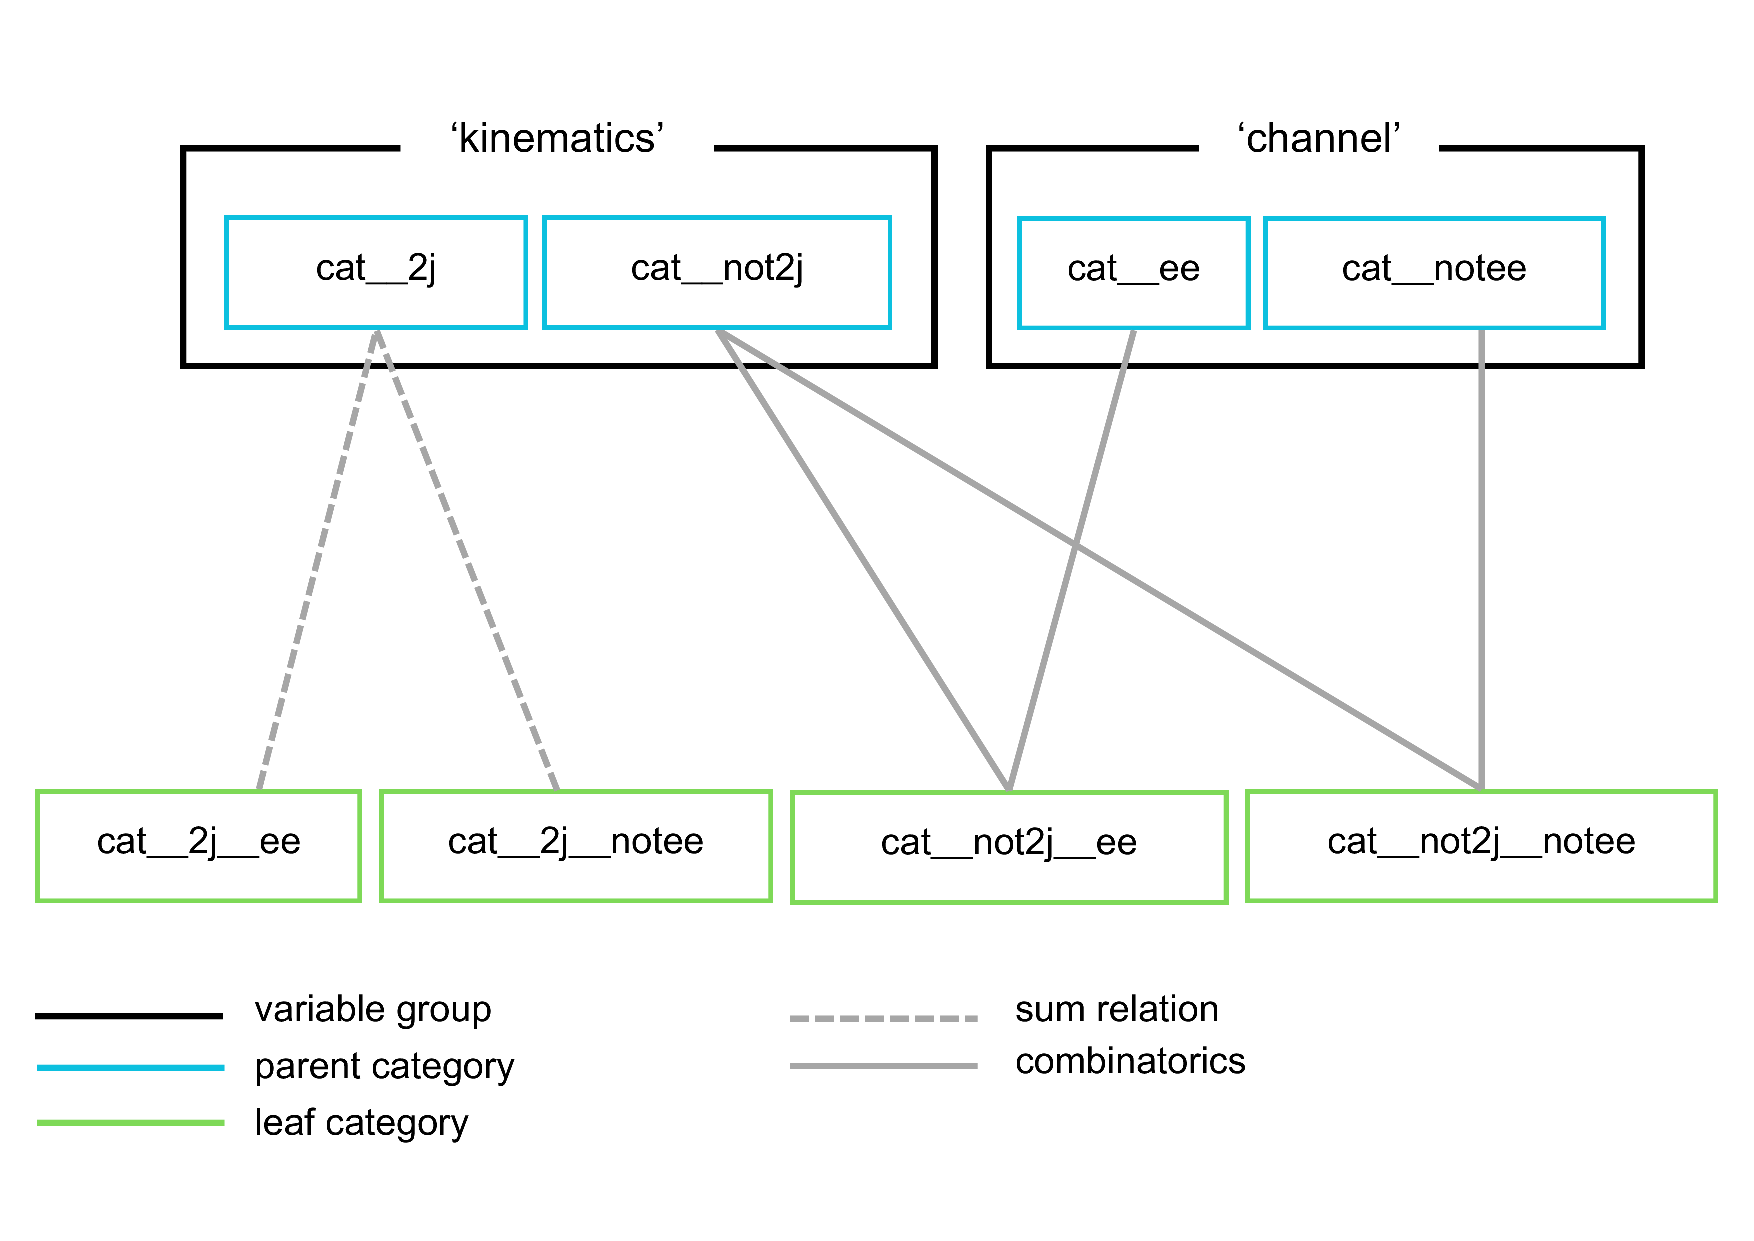
\includegraphics[width=\textwidth]{images/categories.pdf}
    \caption{Example of category combinatorics within ColumnFlow. The variable groups are defined to be orthogonal. Within each variable group, the parent categories are defined so as to cover the whole phase-space and also be orthogonal among themselves. The solid grey lines represent two examples of how parent categories combine into distinct leaf categories. The dashed grey lines represent one example on how a parent category is resolved from the sum of its associated leaf categories. In this example, the four leaf categories are orthogonal and, when summed together, span the whole phase-space without double-counting.}
    \label{fig:categories}
\end{figure}
